%% ----------------------------------------------------------------
%% MAIN FILE 
%% ---------------------------------------------------------------- 

% Set up the document
\documentclass[a4paper, 12pt, oneside]{Thesis}  % Use the "Thesis" style
\graphicspath{images/}                          % Location of the graphics files 

% Table configuration packages
\usepackage{array,graphicx}
\usepackage{booktabs}
\usepackage{pifont}
\usepackage{libertine}
\usepackage{tabu}
\usepackage{longtable}
\usepackage{xcolor}
\usepackage{tcolorbox}
\usepackage{textcomp}
\usepackage{multicol}
%\usepackage{amsthm}

\makeatother

% Include any extra LaTeX packages required
\usepackage[square, numbers, comma, sort&compress]{natbib}          % natbib for the bibliography
\usepackage{verbatim}                                               % Needed to make LaTeX comments
\usepackage{float}                                                  % To keep figures in place
\hypersetup{urlcolor=black, colorlinks=false, pdfborder = {0 0 0}}  % Colours hyperlinks in blue

% Define enumerated description lists
\usepackage{enumitem}
\newcounter{descriptcount}
\newcounter{descriptcount2}
\newlist{enumdescript}{description}{2}
\setlist[enumdescript,1]{%
  before={\setcounter{descriptcount}{0}%
          \renewcommand*\thedescriptcount{\arabic{descriptcount}.}}
  ,font=\bfseries\stepcounter{descriptcount}\thedescriptcount~
}
\setlist[enumdescript,2]{%
  before={\setcounter{descriptcount2}{0}%
          \renewcommand*\thedescriptcount{\roman{descriptcount2}.}}
  ,font=\bfseries\stepcounter{descriptcount2}\thedescriptcount~
}
 
% Theorem, propositions and definitions enviroment
% https://www.overleaf.com/learn/latex/theorems_and_proofs

%\newtheorem{theorem}{Theorem}
%\newtheorem{corollary}{Corollary} %[section]
%\newtheorem{lemma}{Lemma}
%\newtheorem{definition}{Definition}
%\newtheorem{proposition}{Proposition}

% Theorem enviroment example
%\begin{theorem}
%Let $f$ be a function whose derivative exists in every point, then $f$ is 
%a continuous function.
%\end{theorem}
%
%\begin{theorem}[Pythagorean theorem]
%\label{pythagorean}
%This is a theorema about right triangles and can be summarised in the %next 
%equation 
%\[ x^2 + y^2 = z^2 \]
%\end{theorem}

 
%% ----------------------------------------------------------------
%% DOCUMENT START
%% ---------------------------------------------------------------- 
\begin{document}

% Configuration and parameters given in  Thesis.cls file
\frontmatter                % Begin the book's numbering; frontpage
%\pagenumbering{arabic}     % In case we don't want roman numbers enumeration at first

%% ----------------------------------------------------------------

\setstretch{1.3}  % Better to have smaller font and larger line spacing than the other way round

% Define the page headers using the FancyHdr package and set up for one-sided printing
\fancyhead{}      % Clears all page headers and footers
\rhead{\thepage}  % Sets the right side header to show the page number
\lhead{}          % Clears the left side page header

\pagestyle{fancy}  % Finally, use the "fancy" page style to implement the FancyHdr headers

%% ----------------------------------------------------------------
%% TITLE PAGE
%% ---------------------------------------------------------------- 

\title  {GRAVER BASIS}

\authors  {\texorpdfstring
            {\href{mailto:francisco.blazquezmartinez@epfl.ch}{Francisco Javier Blázquez Martínez}}
            {Francisco Javier Blázquez Martínez}
            }
\addresses  {\groupname\\\deptname\\\univname}  
\date       {\today}
\subject    {}
\keywords   {}

\maketitle



%% ----------------------------------------------------------------
%% DECLARATION OF AUTHORSHIP
%% ---------------------------------------------------------------- 

\begin{comment}
\Declaration{

\addtocontents{toc}{\vspace{1em}}  % Add a gap in the Contents, for aesthetics

I, Francisco Javier Blázquez Martínez, declare that this thesis titled ``Graver basis'' and the work presented in it are my own. I confirm that:

\begin{itemize} 
\item[\tiny{$\blacksquare$}] This work was done wholly or mainly while in candidature for a research degree at this University.
 
\item[\tiny{$\blacksquare$}] Where any part of this thesis has previously been submitted for a degree or any other qualification at this University or any other institution, this has been clearly stated.
 
\item[\tiny{$\blacksquare$}] Where I have consulted the published work of others, this is always clearly attributed.
 
\item[\tiny{$\blacksquare$}] Where I have quoted from the work of others, the source is always given. With the exception of such quotations, this thesis is entirely my own work.
 
\item[\tiny{$\blacksquare$}] I have acknowledged all main sources of help.
 
\item[\tiny{$\blacksquare$}] Where the thesis is based on work done by myself jointly with others, I have made clear exactly what was done by others and what I have contributed myself.
\\
\end{itemize}
 
 
Signed:\\
\rule[1em]{25em}{0.5pt}  % This prints a line for the signature
 
Date:\\
\rule[1em]{25em}{0.5pt}  % This prints a line to write the date
}
\clearpage  % Declaration ended, now start a new page
\end{comment}
%% ----------------------------------------------------------------
%% QUOTE PAGE
%% ---------------------------------------------------------------- 
\begin{comment}
\pagestyle{empty}  % No headers or footers for the following pages

\null\vfill
% Now comes the "Funny Quote", written in italics
\textit{Inspiring quote goes here (optional)}

\begin{flushright}
Quote's attribution
\end{flushright}

\vfill\vfill\vfill\vfill\vfill\vfill\null
\clearpage  % Funny Quote page ended, start a new page
\end{comment}

%% ----------------------------------------------------------------
%% ABSTRACT PAGE
%% ---------------------------------------------------------------- 
\begin{comment}
% We can modify the abstract style in thesis.cls file!
\addtotoc{Abstract}  % Add the "Abstract" page entry to the Contents
\abstract{
\addtocontents{toc}{\vspace{1em}}  % Add a gap in the Contents, for aesthetics

Abstract goes here.

}

\clearpage  % Abstract ended, start a new page
\end{comment}
%% ----------------------------------------------------------------
%% DEDICATION
%% ---------------------------------------------------------------- 
%\begin{comment}
% Insert empty page / blank page
%\thispagestyle{empty}
%\null
%\newpage

% TODO: Improve expressivity
% Joaquín: For showing me what real maths were 
% Parents: For showing me further than maths

\pagestyle{empty}  % Page style needs to be empty for this page
\dedicatory{
To my brother Joaquín, for showing me what mathematics were during dinners at home.\\
\vspace{1cm}
To my parents, for teaching me beyond the scope of mathematics.\\
}

\addtocontents{toc}{\vspace{2em}}  % Add a gap in the Contents, for aesthetics
%\end{comment}

%% ----------------------------------------------------------------
%% ACKNOWLEDGEMENTS
%% ---------------------------------------------------------------- 
\setstretch{1.3}  % Reset the line-spacing to 1.3 for body text (if it has changed)

% The Acknowledgements page, for thanking everyone
\acknowledgements{
\addtocontents{toc}{\vspace{1em}}  % Add a gap in the Contents, for aesthetics

% TODO: Improve!
First and foremost I would like to express my sincere thanks to Jana Cslovjecsek for helping me throughout the whole project as well as to Professor Friedrich Eisenbrand for giving me the oportunity of doing this. It has been a very didactic experience that I really appreciate.

Moreover, this project is one of my finals steps for obtaining the Double degree in Mathematics-Computer Engineering at Complutense University of Madrid that, thanks to the help of many people, I have been able to carry out in this fantastic university that is the École Politechnique Fédéreale de Lausanne.  I want to expressly thank Prof. Katzalin Olcoz and Prof. Daniel Chaver for all the facilities and help. I can't help but be grateful to the Complutense University and all the teachers I've had for everything I have learnt.

% TODO: Prof. for Katzalin and Daniel?
% TODO: I can't help but be grateful?

Finally I would like to thank my family for their unconditional support and also Luis Felipe Ramirez, for advising me so well in the important decisions these last years.  

To all, thank you very much from the heart.

% TODO: Luis Felipe's surname!

% Schema:
%-----------------------
% Jana Cslovjecsek
% Friedrich Eisenbrand

% Daniel Cháver
% Katzalin Olcoz
% David Atienza
% Jana Cslovjecsek
% Friedrich Eisenbrand

% Complutense University
% EPFL

% Parents
% Luis Felipe!

}
\clearpage  % End of the Acknowledgements

\pagestyle{fancy}  %The page style headers have been "empty" all this time, now use the "fancy"

%% ----------------------------------------------------------------
%% INDEX
%% ---------------------------------------------------------------- 

% TODO: I don't like subsections in the index!!

\lhead{\emph{Contents}}  % Set the left side page header to "Contents"
\tableofcontents  % Write out the Table of Contents

%% ----------------------------------------------------------------
%% LIST OF FIGURES
%% ---------------------------------------------------------------- 
\begin{comment}
\lhead{\emph{List of Figures}}  % Set the left side page header to "List if Figures"
\listoffigures  % Write out the List of Figures
\end{comment}

%% ----------------------------------------------------------------
%% LIST OF TABLES
%% ---------------------------------------------------------------- 
\begin{comment}
\lhead{\emph{List of Tables}}  % Set the left side page header to "List of Tables"
\listoftables  % Write out the List of Tables
\end{comment}

%% ----------------------------------------------------------------
%% ABBREVIATIONS
%% ---------------------------------------------------------------- 
\begin{comment}
\setstretch{1.5}  % Set the line spacing to 1.5, this makes the following tables easier to read
\clearpage  % Start a new page
\lhead{\emph{Abbreviations}}  % Set the left side page header to "Abbreviations"
\listofsymbols{ll}  % Include a list of Abbreviations (a table of two columns)
{
\textbf{Acronym} & \textbf{W}hat (it) \textbf{S}tands \textbf{F}or \\
% Abbreviations go here
}

\lhead{}

\setstretch{1.3}  % Return the line spacing back to 1.3

\end{comment}

%% ----------------------------------------------------------------
%% INCLUDE ALL SECTIONS
%% ---------------------------------------------------------------- 
\mainmatter	       % Begin normal, numeric (1,2,3...) page numbering
\pagestyle{fancy}  % Return the page headers back to the "fancy" style

% Include the chapters of the thesis, as separate files
% Just uncomment the lines as you write the chapters

\chapter{Introduction} \label{introduction}

\lhead{\emph{Introduction}}  % Set the left side page header to "Contents"
%\rhead{\emph{Introduction}}  % Set the right side page header

% Present the IP problem
Hereafter, the underlying problem is the classical \textit{Integer program} (IP), that we formulate in the following way:
\begin{equation*}
    % TODO: Maybe call it IP_A(b,c)??
    (IP) \equiv max\{c^tx : Ax = b, l \leq x \leq u, x \in \mathbb{Z}^n \}
\end{equation*}
\vspace{-50pt}
\begin{center}
$A \in \mathbb{Z}^{mxn}$, $b \in \mathbb{Z}^m$, $c \in \mathbb{Z}^n$, $l$  and $u$ lower and upper bounds for x
\end{center}

% Simplicity: Not allowing non-linear restrictions/objective functions
% Powerful: Lot of applications, many problems admit IP formulation
% Problem: Is NP-Complete
% Solution (+-): Techniques for certain IPs, GRAVER BASIS!
% N-Fold: As a success example

Despite the simplicity of its formulation, allowing only linear constraints and a linear objective function, it's well known the importance of IP. A large number of problems in diverse fields of the mathematics and algorithms (with an infinity of applications) admit an IP formulation. Unfortunately, it's also well known that IP is NP-Complete, what means that no efficient algorithm is likely to exist for solving the IP in the general case. This explains the great interest in restricted formulations of the problem and in certain resolution techniques (even when they can't be applied to the general IP). In the following sections we present the last techniques based on the \textbf{Graver bases} and its bounds as well as their application to the \textbf{N-Fold IP}, a restricted formulation of the IP which has won relevance in the last decades given its theoretical properties and its wide applications. 

% One of this techniques is decomposing the constraint matrix into block structure which has proved useful for IP formulations where this matrix is sparse or has a certain shape.

% TODO: Improve the end of the paragraph!
For this purpose, we first introduce the Graver basis of a given matrix, explore its properties, bounds, and how can these be applied for solving the general IP. We then study the N-Fold case and show, with the help of Graver bases, that the N-Fold IP can be solved in polynomial time. In the last sections we go further improving this polynomial complexity, obtaining two different efficient algorithms. One based on augmenting a feasible solution and another based on a proximity bound. 

%and show how applying these Graver Basis techniques (and specially its bounds) we can restrict the search of an improvement direction at a feasible point or even directly restrict the search of an optimal solution at a solution of the linear relaxation. All together lead us to a polynomial and efficient algorithm for this kind of problems.


% We could add much more here if needed:
%
% We can briefly introduce each section/chapter
% Explicit references to Graver Basis appearance
% Explicit references to N-Fold appearance
% Explicit general techniques for IP
% Explicit specific techniques for restricted IP








 % Introduction

\chapter{Graver bases} \label{literature}

\lhead{\emph{Graver bases}}  % Set the left side page header


Before introducing the concept of Graver basis of a matrix, we define a partial order $\sqsubseteq$ in $\mathbb{R}^n$ by $u \sqsubseteq v$ if $u_i \cdot v_i \geq 0$ and $|u_i| \leq |v_i|$ for all i. Note that the condition $u_i \cdot v_i \geq 0$ means that $\sqsubseteq$ can only compare \textit{sign compatible} vectors, i.e., with the same sign componentwise. The Graver basis of a matrix is the set of minimal elements (for this order $\sqsubseteq$) in its integral kernel excluding zero. Formally: 

\begin{definition}[\textbf{Graver basis}]
The Graver basis ($\mathcal{G}(A)$) of a given matrix $A \in \mathbb{Z}^{mxn}$ is defined as the set of $\sqsubseteq$-minimal elements in $\{z \in \mathbb{Z}^n: Az = 0, z\neq0\}$.%$ker(A) \setminus \{0\}$.\\
\end{definition}

\vspace{-5pt}
Graver bases were initially defined as \textit{universal integral test set} in \cite{GRAVER:1975} by Jack. E. Graver, in 1975. They often appear also defined in an equivalent way as the nonzero indecomposable elements in $ker(A)$. Indecomposable in the sense that they can not be expressed as the sum of two sign compatible vectors. It's easy to see the equivalence of both definitions.

Now that Graver bases are formally defined, we present their main properties in the form of propositions which will be the theoretical basis for the algorithms presented in the next sections.

\begin{proposition}
For every matrix A, $\mathcal{G}(A)$ is a finite set.
\end{proposition}
\vspace{-20pt}
\begin{proof}
Dickson's lemma states that every subset of $\mathbb{N}^n$ has a finite number of minimal elements (with the order $\leq$ componentwise). It's easy to see that this implies that the integral kernel of A (excluding zero) has a finite number of $\sqsubseteq$-minimal elements in every orthant. As the elements in different orthants are not comparable we have that $\mathcal{G}(A)$ is the union of $2^n$ finite sets, concluding the proof.
\end{proof}

Unfortunately, the cardinality of $\mathcal{G}(A)$ may be exponential in $n$, the number of columns of $A$. This of course limits the explicit computation and usage of the Graver basis to only certain cases but of course doesn't limit its theoretical properties. The most important of these properties is expressed in the following proposition:

\begin{proposition}
Every integral element in $ker(A)$ can be expressed as positive integral linear combination of sign compatible elements in $\mathcal{G}(A)$.
\end{proposition}
\vspace{-20pt}
% TODO: Review!
% TODO: Compare with proof of lemma 4.2 [Onn-Convex_IP-2007]!
\begin{proof}
The proof is by induction in the $\ell_1$ norm. For the base case we see that given $u \in \mathbb{Z}^n\cap ker(A)$ such that $||u||_1 = 1$ then $u$ belongs to $\mathcal{G}(A)$ and the result holds.

For the induction case lets suppose the result is given up to k and take $u \in \mathbb{Z}^n\cap ker(A)$ such that $||u||_1 = k$. Again, if $u$ is minimal in $\mathbb{Z}^n\cap ker(A) \setminus \{0\}$ the result is clear so let's suppose this is not the case. Therefore it exists $u_1$ s.t. $u_1 \sqsubseteq u, u_1 \neq u$. We take $u_2 = u - u_1$. Note that thanks to the definition of $\sqsubseteq$ $u$, $u_1$ and $u_2$ are sign compatible and thanks to $u \neq u_1$ necessarily  $||u_1||_1,||u_2||_1 \leq k$. With this appreciations, the proof concludes after applying the induction hypothesis:\\
\vspace{-30pt}
\begin{center}
    $u = u_1 + u_2 = \sum \alpha_{1i}g_{1i} + \sum \alpha_{2i}g_{2i} = \sum \alpha_{j}g_{j}$
\end{center}
\end{proof}

This proposition is the reason why Graver bases were introduced as \textit{universal integral test set}. It ensures that, given any feasible point, the whole feasible region can be expressed in terms of elements in $\mathcal{G}(A)$. Note that thanks to requiring positive coefficients and sign compatible elements we avoid cancellations in every component. 

In the next proposition we see how, thanks to this property, we can do an optimality test for any feasible point using only elements in the Graver basis.

\begin{proposition}
Given a feasible point $z$ of the IP, $z$ is not optimum if and only if there exists $g \in \mathcal{G}(A)$ s.t. $c^tg > 0$ and $l \leq z + g \leq u$.
\end{proposition}
\vspace{-20pt}
\begin{proof}
If there exists $g \in \mathcal{G}(A)$ (therefore $\in ker(A)$) $s.t. c^tg > 0$ is clear that $z + g$ is a feasible point which strictly improves the objective function, so $z$ is not an optimum. 

For the other implication, if z is not an optimum we can take a feasible point $y$ improving $z$, then $y - z$ verifies the hypothesis of the previous proposition so there exist $g_i \in G(A)$, $\alpha_i \geq 0$ s. t. $0 < c^t(y - z) = \sum \alpha_i c^t g_i$ and it's then clear that exists at least one $g_i \in \mathcal{G}(A)$ verifying $c^tg_i > 0$. Finally, thanks of $\alpha_i \geq 0$ and $g_i$ being sign compatible with $y - z$ we have that for all $i$, $l \leq z \leq z + g_i \leq z + \sum \alpha_i g_i = y \leq u$.
\end{proof}

\section{Graver Basis greedy augmentation algorithm}

We now consider how to solve the general IP with the help of Graver bases. Note that proposition 2.4 doesn't only give us an optimality test but also provide us an improvement direction if the feasible point is not optimal. We can follow that improvement direction to get a better feasible point and then repeat this process. That is the idea of the following procedure (idea introduced in \cite{GRAVER:1975}):

\textbf{General IP algorithm using Graver basis}
\vspace{-8pt}
\begin{enumerate}
    \item From a feasible solution $z_i$
    \item Find $g^*$ optimum for the sub-problem: \vspace{4pt}\\
          $max\{c^tg : g \in \mathcal{G}(A), l \leq z_i + g \leq u \}$ \vspace{4pt}
    \begin{itemize}
        \item $c^tg^* \leq 0 \implies z_i$ optimal solution.
        \item $c^tg^* > 0 \implies$ $g^*$ improvement direction, loop back to 1 with:\\ $z_{i+1} = z_i + \lambda \cdot g^*$ with the biggest $\lambda$ respecting the bounds.
    \end{itemize}
\end{enumerate}
%\hspace{15pt} [References??]

We can affirm that it's an algorithm, i.e., it finishes in a finite number of steps, thanks to the lower and upper bounds $l$ and $u$. We can assume they are finite and, this way, the objective function is also bounded. Since every iteration we are strictly increasing the objective function, no infinite loop is possible. As is well known, it is always possible to add suitable polynomial upper and lower bounds without excluding some optimal solution if any, so assuming $l$ and $u$ to be finite is no loss of generality.

% TODO: href style!
% TODO: Maybe proposition with the complexity ??
% TODO: Improve \cite{...} (Theorem x.y) ??
The question that arises now is the complexity of this algorithm. It was analyzed in \cite{LHOW:2006} (Theorem 3.3) showing that it's polynomial. This of course doesn't mean we have a polynomial algorithm for the general IP, it means that, given an IP along with its Graver basis, we have a polynomial algorithm in this input size. The complexity of the problem remains in computing the Graver basis which, as we announced, may be exponential. This makes the algorithm non-viable but for small matrices. In the Appendix A we go further to analyze how to compute the Graver basis of a given matrix and we introduce the tool \href{https://4ti2.github.io/}{4ti2}.

% TODO: Textbf for the complexity (last sentence) ??
Another way to estimate the complexity of the algorithm is using \cite{HOW:2009} (Theorem 2.b), which states that the number of augmentation steps is polynomial. Since once obtained the Graver basis the cost of each augmentation step is in the order $n \cdot |\mathcal{G}(A)|$ (search over $\mathcal{G}(A)$), it's clear that the algorithm is polynomial in $n \cdot |\mathcal{G}(A)|$.



\section{Graver Basis norm bounds}

Up to this point we have seen how Graver bases allow a straightforward algorithm for the general IP. However, we have seen that its main drawback is that it requires the explicit computation of the Graver basis. In this section we show how we can avoid computing it thanks to bounds on the $\ell_1$-norm of the Graver basis elements.

\begin{proposition}[\textbf{Graver basis bounds}]
Given $A \in \mathbb{Z}^{mxn}$ and $\Delta$ an upper bound for the absolute value of each component of $A$, for every $g \in \mathcal{G}(A)$:
\vspace{-10pt}
\begin{itemize}
    \item $||g||_1 \leq m^{m/2}\Delta^m\cdot(n - m)$ \hspace{10pt}[Onn 2010]
    \item $||g||_1 \leq (2m \Delta + 1)^m$ \hspace{41pt}[Eisenbrand,Hunkenschröder,Klein 2018]
\end{itemize}
\end{proposition}

We refer to \cite{ONN:2010} and \cite{EISENBRAND:2018} for the proof. Note that both bounds are exponential in the number of rows of $A$ but the second one has the advantage of being independent in the number of columns. 

Why should bounds to the Graver bases help? Because thanks to Proposition 2.4, the search of an improvement direction can be restricted to the elements in the Graver basis and, thanks to the bounds, we can restrict our search space without excluding any element of the Graver basis. This is the idea of the following algorithm (see \cite{HEMMECKE:2011}).

% TODO: Maybe here is the place for the first image!
% TODO: Definitely it would be nice to add the images!

\vspace{10pt}
\begin{figure}[h]
\centering
\begin{minipage}[b]{0.45\textwidth}
    \centering
    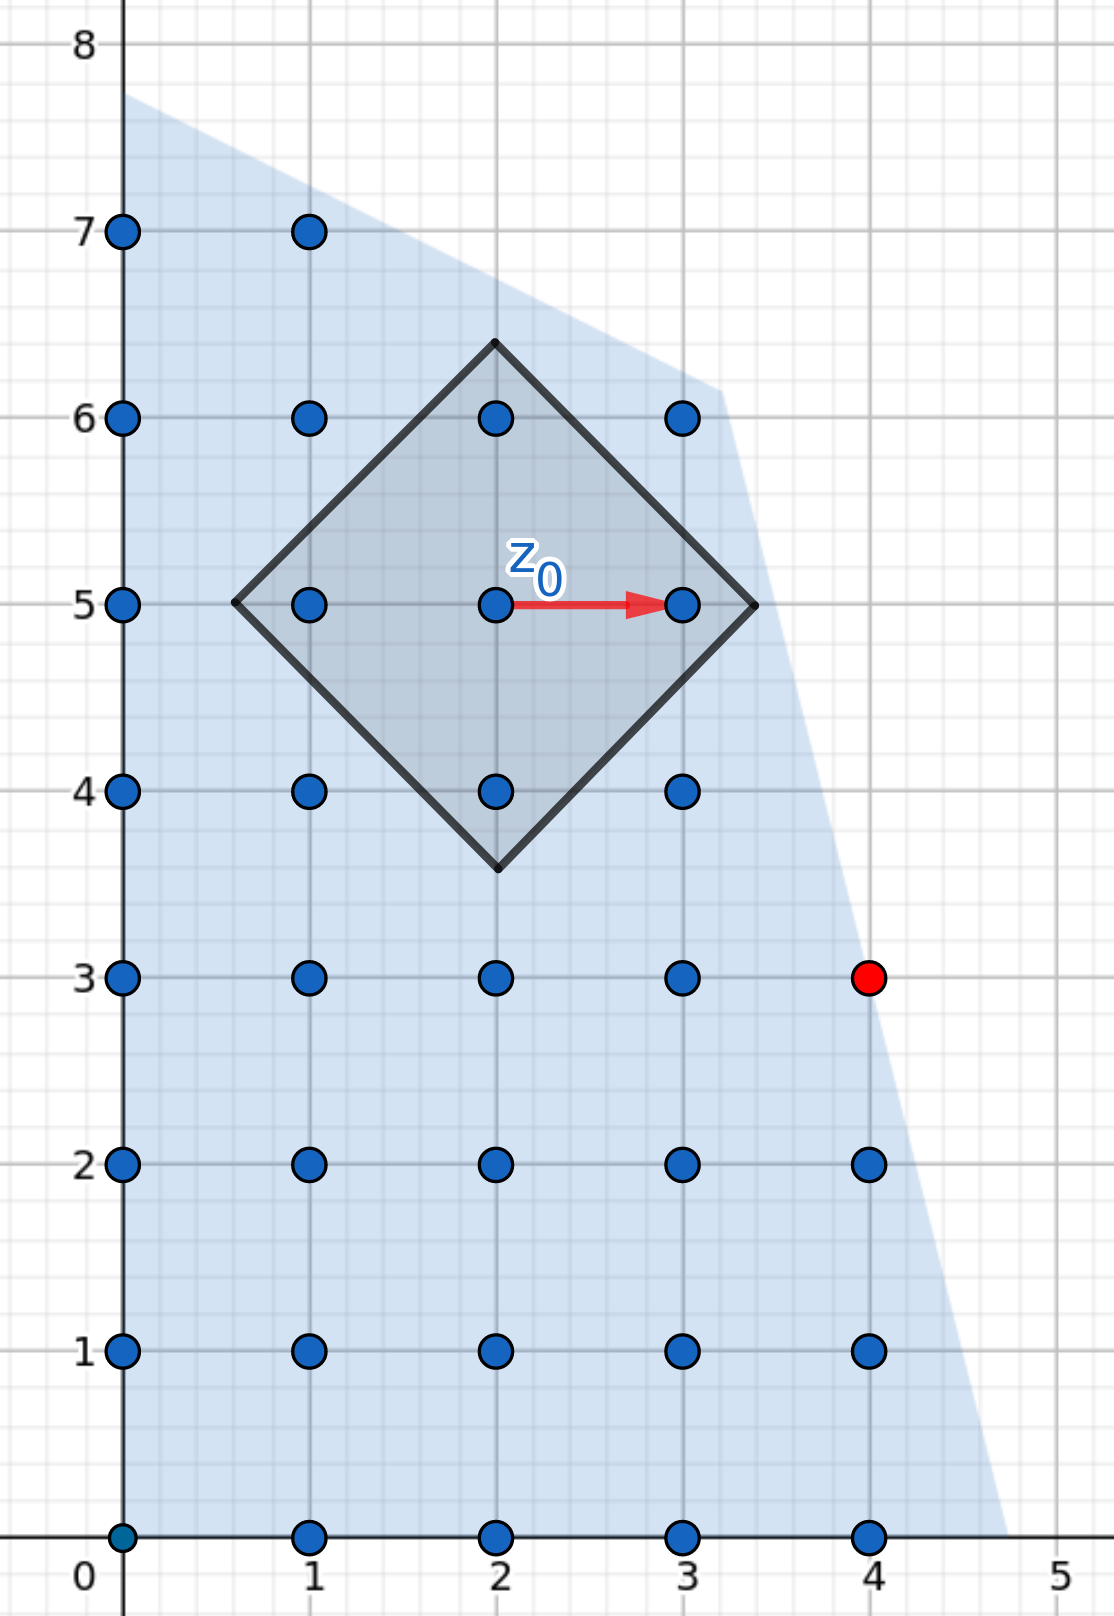
\includegraphics[width=0.9\textwidth]{images/IP(6).png}
    % TODO!
    \caption{Complete this}
\end{minipage}
\hfill
\begin{minipage}[b]{0.45\textwidth}
    \centering
    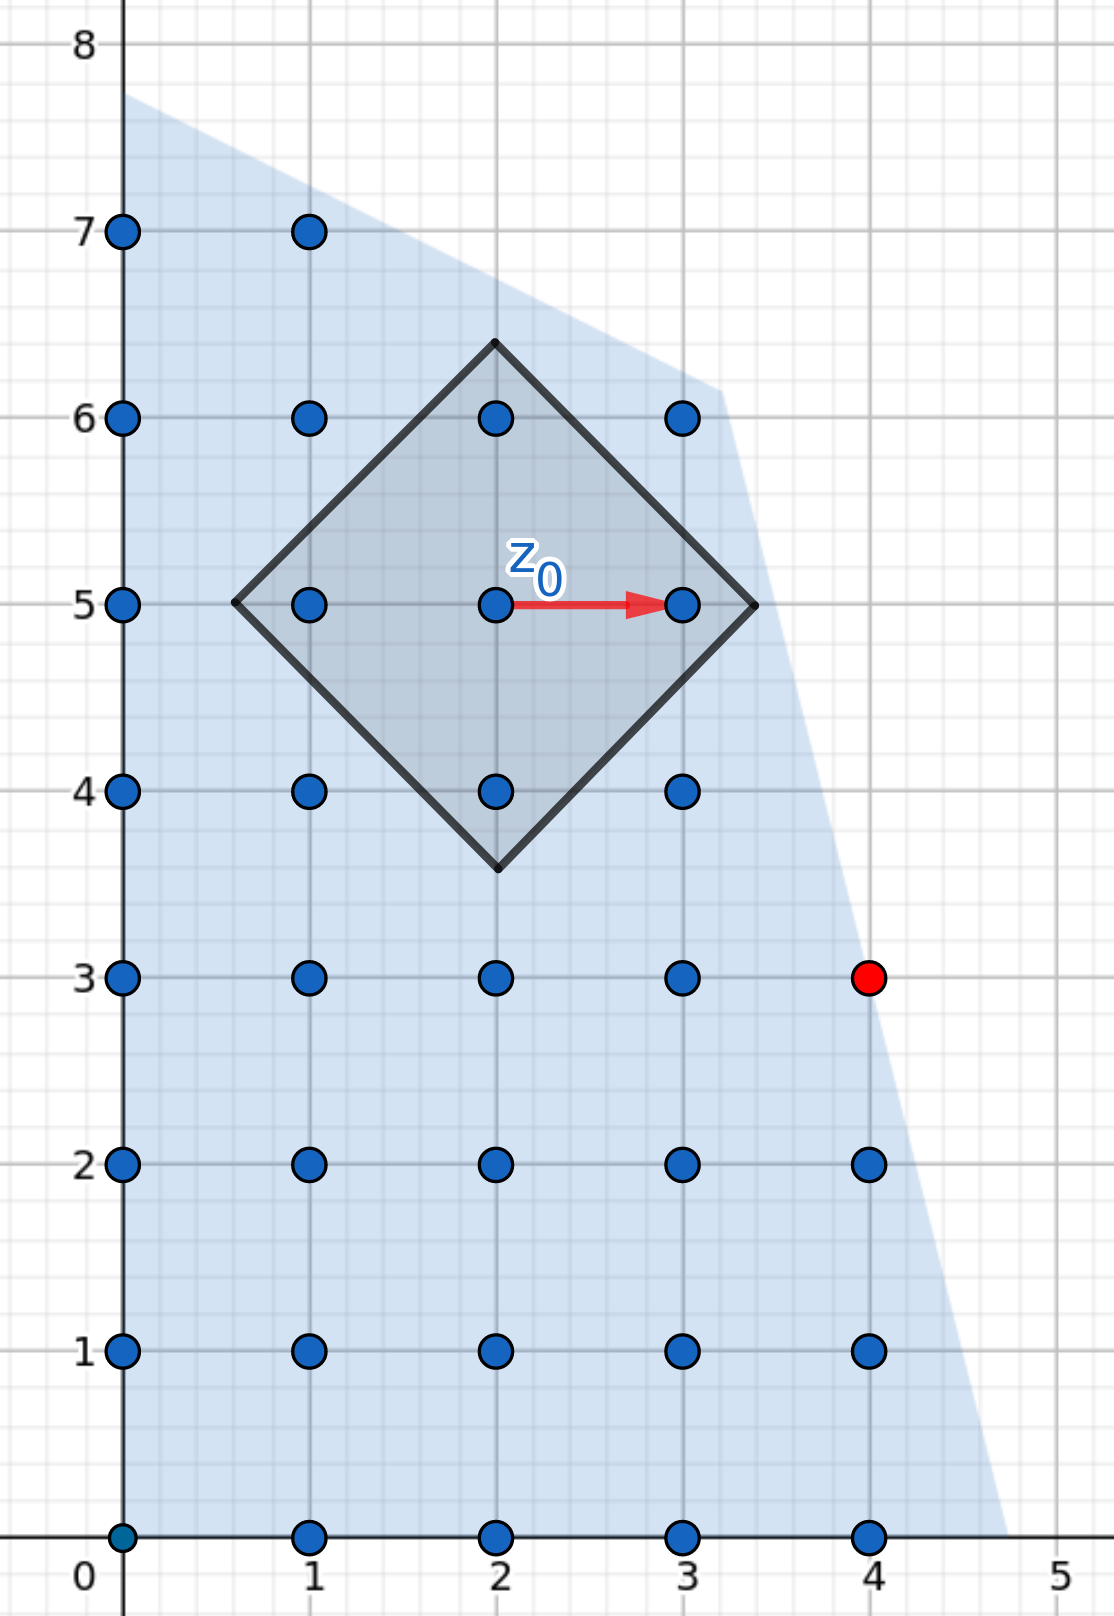
\includegraphics[width=0.9\textwidth]{images/IP(6).png}
    % TODO!
    \caption{Also this}
\end{minipage}
\end{figure}

% TODO: I don't like newpage commands! avoid if possible
\newpage
\textbf{General IP algorithm using Graver basis norm bound}
\vspace{-8pt}
\begin{enumerate}
    \item From a feasible solution $z_i$
    \item Find $g^*$ optimum for the sub-problem: \vspace{4pt}\\
          $max\{c^tg : Ag = 0, l-z_i \leq g \leq u-z_i, g \in \mathbb{Z}^n, ||g||_1 \leq ||\mathcal{G}(A)|| \}$ \vspace{4pt}
    \begin{itemize}
        \item $g^* = 0 \implies z_i$ optimal solution.
        \item $g^* \neq 0 \implies$ $g^*$ improvement direction, loop back to 1 with:\\
        $z_{i+1} = z_i + \lambda \cdot g^*$ with the biggest $\lambda$ respecting the bounds.
    \end{itemize}
\end{enumerate}
%\hspace{15pt} [Hemmecke, Onn, Romanchuk 2013]


As we advanced, the main advantage of this algorithm is that it doesn't require the explicit computation of the Graver Basis. However, the complexity is totally dependent on the added restriction $||g||_1 \leq ||\mathcal{G}(A)||$, and the only bounds we have for the general case are exponential. In this case, the additional restriction to the problem doesn't improves the lower and upper bounds and the complexity is exponential. 

In certain cases we can get a much tighter bound for the Graver Basis elements and this can help us to get a faster algorithm. The N-Fold IP is an iconic example.  % Graver Basis definition and properties

\chapter{N-Fold IP} \label{3.N-Fold}
\lhead{\emph{N-Fold IP}}  

% N-Fold introduction and notation
A generalized \emph{N-Fold IP} has constraint matrix A of the form ($A_i \in \mathbb{Z}^{rxt}, B_i \in \mathbb{Z}^{sxt}$):\\
\begin{equation*} \label{NFold_matrix}
\mathcal{N} = 
\begin{pmatrix}
A_1 & A_2 & \cdots & A_n \\
B_1 & 0   & \cdots & 0 \\
0   & B_2 & \cdots & 0 \\
\vdots    & \vdots & \ddots & \vdots  \\
0   & 0   & \cdots & B_n 
\end{pmatrix}
\end{equation*}


It was presented in \cite{LHOW:2006} in 2006 in a simplified version in which $\forall i,j$  $A_i = A_j, B_i = B_j$. This simplified N-Fold matrix is totally determined given $A \in \mathbb{Z}^{r \times t}$, $B \in \mathbb{Z}^{s \times t}$ and the order $n$ and we denote it by $N_{A,B}^{(n)}$. Hereafter, we'll refer to the generalized formulation as \emph{N-Fold IP}. 

% N-Fold relevance
The \emph{N-Fold IP} has a wide range of applications. In \cite{LHOW:2006} it's applied to the multiway transportation and cutting-stock problems and in \cite{HEMMECKE:2011} to privacy and disclosure control in
statistical databases just to name a few examples beyond the typical in operations research. In fact, the \emph{N-Fold IP} is universal. Every IP can be expressed as an \emph{N-Fold IP}. This is because, as shown in \cite{LO:2006}, every IP can be modeled as a slim 3-way transportation program, which can be expressed as an \emph{N-Fold IP}. However, this is more a theoretical achievement which shows the expressiveness power of the N-Fold rather than a useful practical approach for solving any IP. 

In any case, the \emph{N-Fold IP} is interesting by itself since it has good theoretical properties. In the following sections we will study it with the help of Graver bases to finally obtain a roughly linear algorithm for its resolution. We start with the following proposition:

% PROPERTIES
% N-Fold graver basis is polynomial
\begin{theorem} \label{Nfold_GB_computation_polynomial}
Fixed any $A \in \mathbb{Z}^{r \times t}$ and $B \in \mathbb{Z}^{s \times t}$, there is an algorithm polynomial in $n$ that computes the Graver basis of the N-Fold matrix $N_{A,B}^{(n)}$. 
\end{theorem}
\vspace{-10pt}

We won't go into the details of the proof of this proposition, they can be seen in \cite[Theorem 4.2]{LHOW:2006}. However, we consider important to remark that this proposition implies that, fixed $A$ and $B$, the cardinality of $\mathcal{G}(N_{A,B}^{(n)})$ is bounded by a polynomial function of $n$.

This has an important consequence, the greedy Graver basis augmentation algorithm presented before has, in this case, polynomial complexity for every augmentation step and therefore polynomial complexity. However it's still remaining the problem of obtaining an initial feasible solution. That is precisely what solves the next proposition:

% Two phase method for N-Fold
\begin{lemma} \label{Nfold_two_phase}
Fixed any $A \in \mathbb{Z}^{r \times t}$ and $B \in \mathbb{Z}^{s \times t}$, there is an algorithm polynomial in $n$ that, given a  demand vector $b \in \mathbb{Z}^{s + nr}$, either finds a feasible point $x \in \mathbb{Z}^{nt}$ to the simplified \emph{N-Fold IP} of order n, or asserts that no feasible solution exists.
\end{lemma}
\vspace{-15pt} 
\begin{proof}
This is a result proved in \cite[Lemma 5.2]{LHOW:2006}. The idea is that we can add $2n(s+r)$ artificial variables to construct an \emph{N-Fold IP} for which an initial feasible solution is trivial for any right side $b$. The constraint matrix would result as below: 
\vspace{5pt}
\begin{equation*}
N = 
\setcounter{MaxMatrixCols}{20}
\begin{pmatrix}
A & I_s & -I_s & 0 & 0 & A & I_s & -I_s & 0 & 0 & \cdots & A & I_s & -I_s & 0 & 0 \\
B & 0 & 0 & -I_r & I_r & 0 & 0 & 0 & 0 & 0 & \cdots & 0 & 0 & 0 & 0 & 0 \\
0 & 0 & 0 & 0 & 0 & B & 0 & 0 & -I_r & I_r & \cdots & 0 & 0 & 0 & 0 & 0 \\
\vdots & \vdots & \vdots & \vdots & \vdots & \vdots & \vdots & \vdots & \vdots & \vdots & \ddots & \vdots & \vdots  & \vdots & \vdots & \vdots \\
0 & 0 & 0 & 0 & 0 & 0 & 0 & 0 & 0 & 0 & \cdots & B & 0 & 0 & -I_r & I_r 
\end{pmatrix}
\end{equation*}

This way the result is obtained applying the \textit{two phase method} which, thanks to the previous proposition, runs in polynomial time. Note that we need to add $I$ and $-I$ terms because the artificial variables have to be positive.
\vspace{5pt}
\end{proof}

\begin{theorem}[\textbf{Simplified N-Fold IP is polynomially solvable}]
Fix any pair of integer matrices $A \in \mathbb{Z}^{r \times t}$ and $B \in \mathbb{Z}^{s \times t}$. Then there is a polynomial time algorithm that solves the simplified N-Fold integer programming problem on any input n, b, c.
\end{theorem}
\vspace{-15pt} % TODO: Should be 20
\begin{proof}
Propositions \ref{Nfold_GB_computation_polynomial} and \ref{Nfold_two_phase} ensure that we can compute the  Graver basis of $N_{A,B}^{(n)}$ and a initial feasible point in polynomial time for any $n$, $b$ and $c$. Applying the algorithm \ref{GB_greedy_algorithm} after this solves the problem in global polynomial time.
\end{proof}

% TODO: Maybe too much blank space here!
 % Fundamentals

%\chapter{N-Fold augmentation algorithm} \label{framework}
\section{N-Fold augmentation algorithm}

\begin{lemma}[\textbf{Steinitz Lemma}]
    Let $v_1,...,v_n$ be vectors with $||v_i|| \leq \Delta$ for $i = 1,...,n$. If $\sum_{i=1}^{n} v_i = 0$, then there is a reordering $\pi \in S_n$ such that for each $k \in \{1,...,n\}$ the partial sum $p_k := \sum_{i=1}^{k}v_{\pi(i)}$ satisfies $||p_k|| \leq n\Delta$.
\end{lemma}

It's possible (using Steinitz Lemma) to obtain a much tighter bound for the norm of the elements in the Graver basis than the ones mentioned before. This implies a restriction in the space of search for the improvement direction in the augmentation algorithm making it much faster.

% TODO: Proof?
\begin{lemma}[\textbf{N-Fold Graver basis bound}]
    For all $g \in Gr(N)$ $||g||_1 \leq L_B (2r\Delta L_B + 1)^r =: L_A$ where $L_B = (2s \Delta + 1)^s$
\end{lemma}

% TODO: Proof? At least explanation!
\begin{lemma}[\textbf{N-Fold augmentation algorithm complexity}]
    The N-Fold IP can be solved in time $(nt)^2 log^2(nt) \cdot \varphi (rs\Delta)^{O(r^2s + rs^2)} + LP$
\end{lemma}
\hspace{15pt} [Eisenbrand, Hunkenschröder, Klein 2018]
         % N-Fold augmentation algorithm

% \chapter{N-Fold via LP rounding} \label{platform}
\newpage
\section{N-Fold via LP rounding}  % Set the left side page header

The main drawback for improving the complexity of the augmentation algorithm is that after solving the linear relaxation, we can be arbitrarily far from the optimal solution of the IP, what means that we need many augmentation steps. In this section we follow another approach introduced in \cite{EISENBRAND:2020} based on a more restricted linear relaxation which optimum is closer to the optimum of the IP and we prove this. We then show how to take advantage of this proximity bound to obtain the current fastest algorithm for the N-Fold case, running in roughly linear time.


\subsection{Restricted linear relaxation}
% TODO: Not going deeper but references or really short explanation
\begin{proposition}[\textbf{N-Fold RLR complexity}]
    The N-Fold IP restricted linear relaxation problem can be solved in time
    \begin{equation*}
        O(nt \cdot log^2(nt) \cdot \varphi p(r) (s\Delta)^{O(s^2)})
    \end{equation*}
\end{proposition}

\begin{figure}[h]
\centering
\begin{minipage}[b]{0.45\textwidth}
    \centering
    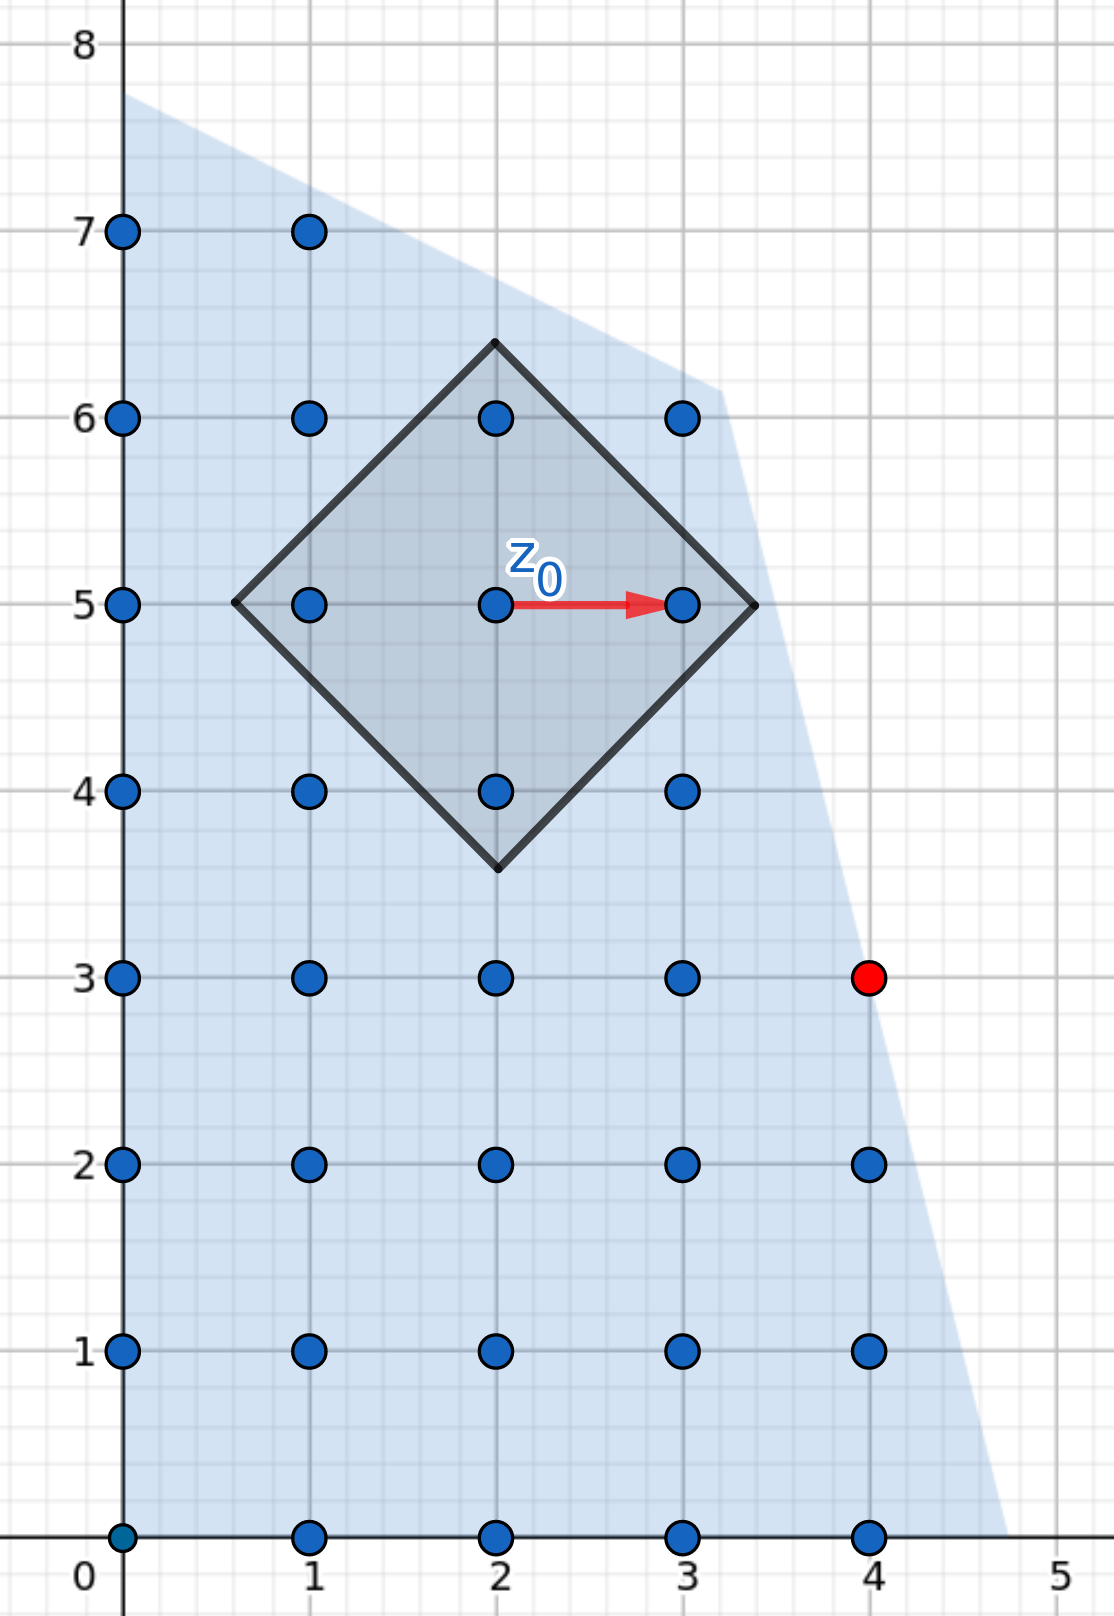
\includegraphics[width=0.9\textwidth]{images/IP(6).png}
    % TODO!
    \caption{Complete this}
\end{minipage}
\hfill
\begin{minipage}[b]{0.45\textwidth}
    \centering
    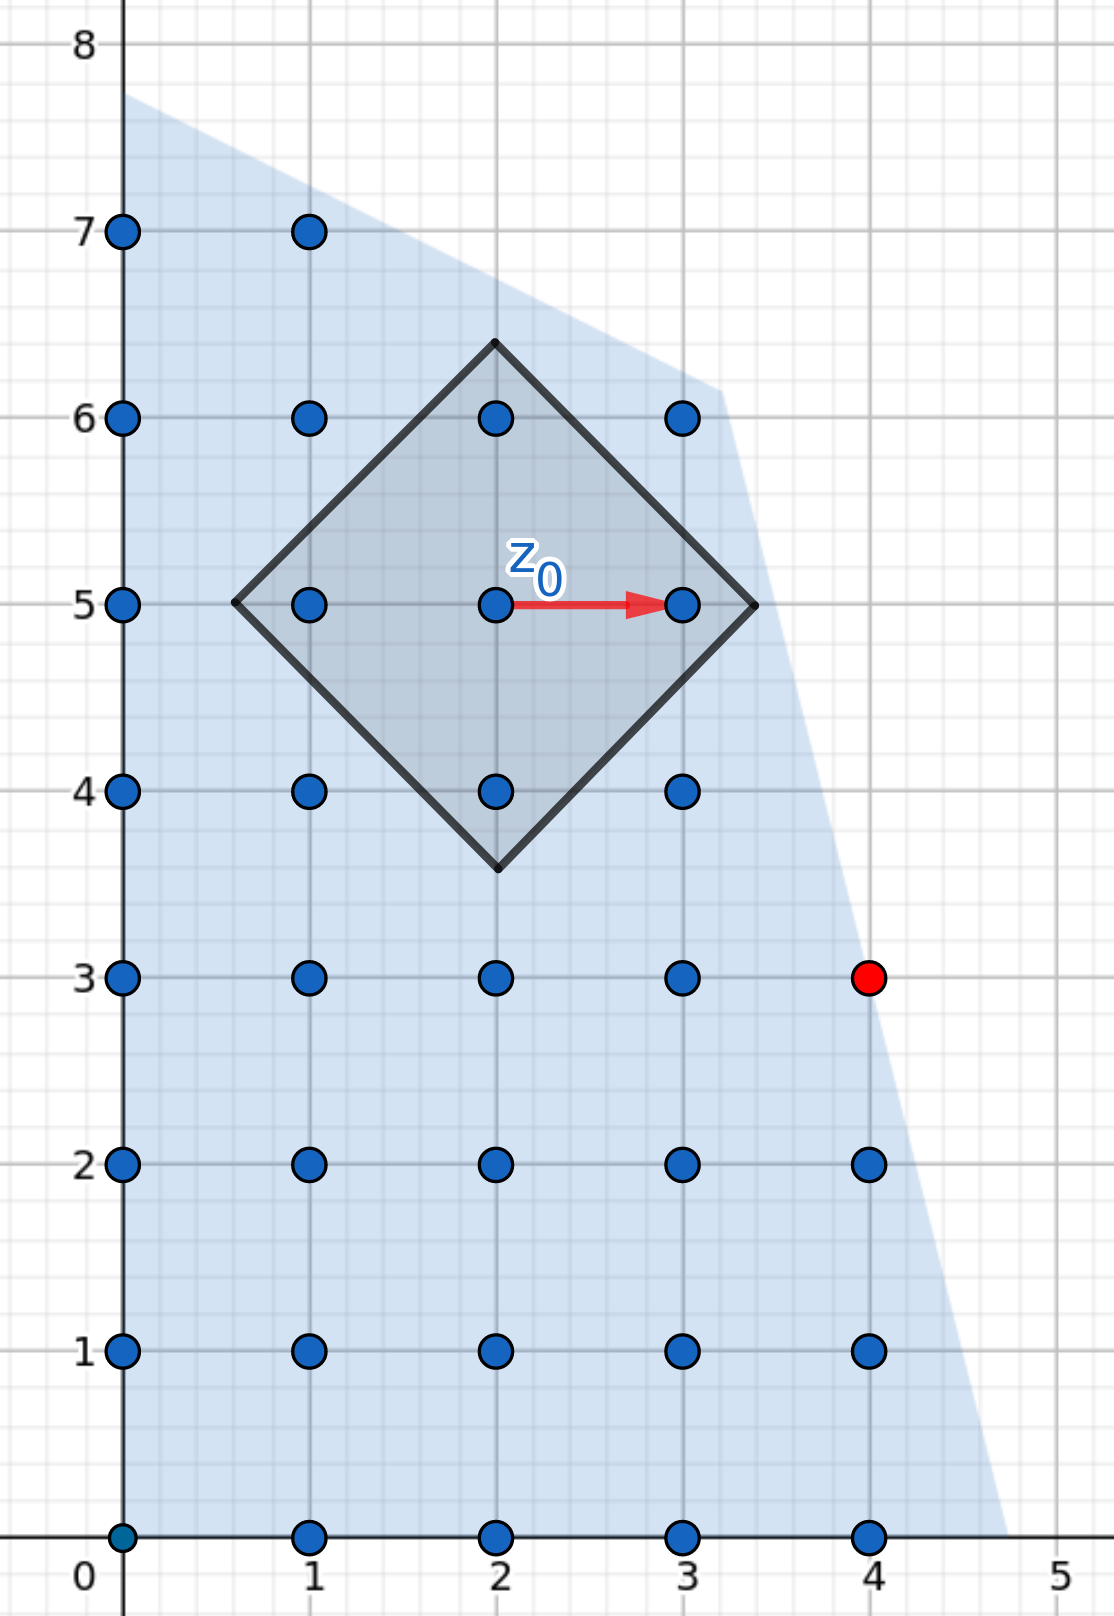
\includegraphics[width=0.9\textwidth]{images/IP(6).png}
    % TODO!
    \caption{Also this}
\end{minipage}
\end{figure}

\newpage
\subsection{Dynamic program}        
% TODO: Proof? At least explanation or references
\begin{proposition}[\textbf{N-Fold RLR to optimum complexity}]
    Given an optimal vertex of an N-Fold RLR, the N-Fold IP can be solved in time
    \begin{equation*}
        O(nt \cdot (rs\Delta)^{O(r^2s+s^2)})
    \end{equation*}
\end{proposition}
%\hspace{15pt}[Cslovjecsek, Eisenbrand, Weismantel 2020]

\begin{proposition}[\textbf{N-Fold proximity to RLR}]
    Let $x^*$ be an optimal vertex solution of a N-Fold RLR, then there exists an optimal solution $z^*$ for the N-Fold IP verifying:  
    \begin{equation*}
        ||z^* - x^*||_1 \leq (rs\Delta)^{O(rs)}
    \end{equation*}
\end{proposition}
\hspace{15pt}[Cslovjecsek, Eisenbrand, Weismantel 2020]



Graph plot for the proof of algorithm complexity:
------------------------------------------------------
\begin{center}
\begin{tikzpicture}[
        > = stealth, % arrow head style
        shorten > = 1pt, % don't touch arrow head to node
        auto,
        node distance = 3cm, % distance between nodes
        semithick % line style
    ]

    \tikzstyle{every state}=[
        draw = black,
        thick,
        fill = white,
        minimum size = 4mm
    ]

    \node[state, minimum size=0.8cm] (s) at (0,0) {$0$};
    
    %\node[state] (w1) at (2,2)  {$y_{11}$};
    %\node[state] (u1) at (2,0)  {$y_{12}$};
    \node[state] (v1) at (2,-2) {$y_{13}$};
    
    %\node (u2) at (4,0)  {$\sum_{i=1}^\ell A_ix^*$};
    \node[state] (w2) at (4,2)  {$y_{21}$};
    %\node[state] (u2) at (4,0)  {$y_{22}$};
    %\node[state] (v2) at (4,-2) {$y_{23}$};
    
    %\node[state] (w3) at (6,2)  {$y_{31}$};
    \node[state] (u3) at (6,0)  {$y_{32}$};
    %\node[state] (v3) at (6,-2) {$y_{33}$};
    
    \node[state] (w4) at (8,2)  {$y_{41}$};
    %\node[state] (u4) at (8,0)  {$y_{42}$};
    %\node[state] (v4) at (8,-2) {$y_{43}$};
    
    \node[state, minimum size=0.8cm] (f) at (10,0)  {$b_0$};
    
    \path[->] (s) edge node  {$c_1^tu_1^*$} (v1);
    \path[->] (v1) edge node {$c_2^tu_2^*$} (w2);
    \path[->] (w2) edge node {$c_3^tu_3^*$} (u3);
    \path[->] (u3) edge node {$c_4^tu_4^*$} (w4);
    \path[->] (w4) edge node {$c_5^tu_5^*$} (f);

    \draw[red, dashed] (1, 3) -- (1, -3);
    \draw[red, dashed] (3, 3) -- (3, -3);
    \draw[red, dashed] (5, 3) -- (5, -3);
    \draw[red, dashed] (7, 3) -- (7, -3);
    \draw[red, dashed] (9, 3) -- (9, -3);
    
    % \node (S1) at (2,-3.5) {$S_1$};
    % \node (S2) at (4,-3.5) {$S_2$};
    % \node (S3) at (6,-3.5) {$S_3$};
    % \node (S4) at (8,-3.5) {$S_4$};
\end{tikzpicture}
\end{center}

Graph plot for the proof of algorithm complexity:
------------------------------------------------------

\begin{center}
\begin{tikzpicture}[
        > = stealth, % arrow head style
        shorten > = 1pt, % don't touch arrow head to node
        auto,
        node distance = 3cm, % distance between nodes
        semithick % line style
    ]

    \tikzstyle{every state}=[
        draw = black,
        thick,
        fill = white,
        minimum size = 4mm
    ]

    \node[state, minimum size=0.8cm] (s) at (0,0) {$0$};
    
    %\node[state] (w1) at (2,2)  {$y_{11}$};
    %\node[state] (u1) at (2,0)  {$y_{12}$};
    \node[state] (v1) at (2,-2) {$y_{13}$};
    
    %\node (u2) at (4,0)  {$\sum_{i=1}^\ell A_ix^*$};
    \node[state] (w2) at (4,2)  {$y_{21}$};
    %\node[state] (u2) at (4,0)  {$y_{22}$};
    %\node[state] (v2) at (4,-2) {$y_{23}$};
    
    %\node[state] (w3) at (6,2)  {$y_{31}$};
    \node[state] (u3) at (6,0)  {$y_{32}$};
    %\node[state] (v3) at (6,-2) {$y_{33}$};
    
    \node[state] (w4) at (8,2)  {$y_{41}$};
    %\node[state] (u4) at (8,0)  {$y_{42}$};
    %\node[state] (v4) at (8,-2) {$y_{43}$};
    
    \node[state, minimum size=0.8cm] (f) at (10,0)  {$b_0$};
    
    \path[->] (s) edge node  {$c_1^tu_1^*$} (v1);
    \path[->] (v1) edge node {$c_2^tu_2^*$} (w2);
    \path[->] (w2) edge node {$c_3^tu_3^*$} (u3);
    \path[->] (u3) edge node {$c_4^tu_4^*$} (w4);
    \path[->] (w4) edge node {$c_5^tu_5^*$} (f);

    \draw[red, dashed] (1, 3) -- (1, -3);
    \draw[red, dashed] (3, 3) -- (3, -3);
    \draw[red, dashed] (5, 3) -- (5, -3);
    \draw[red, dashed] (7, 3) -- (7, -3);
    \draw[red, dashed] (9, 3) -- (9, -3);
    
    % \node (S1) at (2,-3.5) {$S_1$};
    % \node (S2) at (4,-3.5) {$S_2$};
    % \node (S3) at (6,-3.5) {$S_3$};
    % \node (S4) at (8,-3.5) {$S_4$};
\end{tikzpicture}
\end{center}

\textbf{Facts for N-Fold complexity}
\begin{itemize}
    \item $|S_l| \leq (rs\Delta)^{O(r^2s)}$
    \item $|V| + |E| \leq O(n(rs\Delta)^{O(r^2s)})$
    \item The edge IP can be computed in time $t((r + s)\Delta)^{O(r + s)^2}$
    \item Longest path problem in a acyclic digraph can be solved in linear time.
\end{itemize}

\textbf{N-Fold complexity}
\begin{itemize}
\item \textbf{N-Fold complexity}\\
    The N-Fold IP can be solved in time $nt(rs\Delta)^{O(r^2s + s^2)} + RLR$
\end{itemize}
\hspace{15pt}[Cslovjecsek, Eisenbrand, Weismantel 2020] % N-Fold via RLR

%\chapter{Experimentation \& Validation} \label{experimentationANDresults}
 % Experimentation

%\chapter{Conclusions \& Future Work} \label{conclusions}
 % Results and Discussion

%\chapter{Example Appendix} \label{math}
 % Apendix

%% ----------------------------------------------------------------
%% APPENDICES
%% ---------------------------------------------------------------- 
\addtocontents{toc}{\vspace{2em}} % Add a gap in the Contents, for aesthetics

\appendix % Cue to tell LaTeX that the following 'chapters' are Appendices

% Appendix A
\chapter{Graver basis computation with 4ti2} \label{math}

% TODO: Cite
% L. Pottier. Euclide’s algorithm in dimension n. Research report, ISSAC 96, ACM Press, 1996
% R. Hemmecke. On the positive sum property and the computation of Graver test sets. Mathematical Programming 96 (2003), 247–269. 

%@article{article,
%author = {Hemmecke, Raymond},
%year = {2003},
%month = {05},
%pages = {247-269},
%title = {On the positive sum property and the computation of Graver test %sets},
%volume = {96},
%journal = {Math. Program.},
%doi = {10.1007/s10107-003-0385-7}
%} 

% Appendix B
\chapter{IP resolution with Graver Basis example} \label{math}
 

% Example appendices

\addtocontents{toc}{\vspace{2em}}  % Add a gap in the Contents, for aesthetics
\backmatter % End the book's numbering; backpage

%% ----------------------------------------------------------------
%% BIBLIOGRAPHY
%% ---------------------------------------------------------------- 

% References:
% https://www.latex-tutorial.com/tutorials/bibtex/
% https://www.overleaf.com/learn/latex/Bibliography_management_in_LaTeX

\label{Bibliography}
\lhead{\emph{Bibliography}}  % Change the left side page header to "Bibliography"
%\bibliographystyle{plain}
\bibliographystyle{unsrtnat}  % Use the "unsrtnat" BibTeX style for formatting the Bibliography

% TODO: Several warnings in the bibliography!
% TODO: The style can be improved!

\nocite{*}
\bibliography{Bibliography}  % The references (bibliography) information are stored in the file named "Bibliography.bib"

\end{document}  % The End
%% ----------------------------------------------------------------